% 第5章 实验结果与分析

\chapter{实验设计与结果分析}
\label{chap:experiment}

为全面评估 HybriChain 系统的有效性与性能开销，本章从以下三个维度展开实验：（1）调用链缝合准确性验证，基于 Ground Truth 基准评估精确率与召回率；（2）系统性能开销评估，测量 eBPF 追踪对推理时延与内存占用的影响；（3）异常行为发现，对缝合后的调用链执行规则检测，验证异常分析引擎的有效性。

\section{实验环境}

本系统采用 Qwen2-0.5B 与 TinyLlama-1.1B 两款推理引擎作为测试靶点，在 Ollama 0.22.0（Debug 模式）上开展静态符号提取、动态追踪采集与调用链缝合的完整链路实验。表~\ref{tab:env} 给出实验环境配置。

\begin{table}[H]
    \centering
    \caption{实验环境配置}
    \label{tab:env}
    \begin{tabular}{|c|c|}
        \hline
        \textbf{组件} & \textbf{版本/配置} \\
        \hline
        操作系统 & Arch Linux (kernel 7.0.2) \\
        \hline
        推理引擎 & Ollama 0.22.0 (Debug 模式) \\
        \hline
        内核追踪工具 & bpftrace v0.25.1 \\
        \hline
        Go 编译器 & 1.26.2 \\
        \hline
        Python & 3.14.0 \\
        \hline
        TinyLlama-1.1B & 1.1B 参数 \\
        \hline
        Qwen2-0.5B & 0.5B 参数 \\
        \hline
    \end{tabular}
\end{table}

\section{调用链缝合准确性验证}

本节通过人工构建 Ground Truth 基准数据集，评估 HybriChain 缝合算法的精确率、召回率与置信度分布。

\subsection{Ground Truth 基准数据集}

Ground Truth 由源码级调用关系构建。通过对 llama.cpp 源码中的函数调用语句进行静态走读（read/write 调用语句），提取所有必然发生的跨语言调用路径，共计 20 条。这些路径覆盖了以下关键链路：

\begin{itemize}
    \item \textbf{CGO 桥接链路}（5 条）：\texttt{\_cgo\_*\_Cfunc\_llama\_*} $\rightarrow$ \texttt{llama\_*} 系列函数；
    \item \textbf{采样链路}（3 条）：\texttt{llama\_sampler\_sample} $\leftrightarrow$ \texttt{common\_sampler\_sample}；
    \item \textbf{调度计算链路}（5 条）：\texttt{llama\_decode} $\rightarrow$ \texttt{ggml\_backend\_sched\_*} 系列；
    \item \textbf{模型加载链路}（4 条）：\texttt{llama\_model\_load\_from\_file} $\rightarrow$ \texttt{ggml\_*} 系列初始化函数；
    \item \textbf{批量处理链路}（3 条）：\texttt{llama\_batch\_add} $\rightarrow$ \texttt{common\_batch\_add}。
\end{itemize}

\subsection{缝合评估结果}

表~\ref{tab:stitch_eval} 给出了缝合模块在 Ground Truth 基准上的量化评估结果。

\begin{table}[H]
    \centering
    \caption{调用链缝合准确性评估}
    \label{tab:stitch_eval}
    \begin{tabular}{|c|c|p{9.5cm}|}
        \hline
        \textbf{指标} & \textbf{数值} & \textbf{说明} \\
        \hline
        精确率（Precision） & 全部确认 & 缝合确认的全部为正确边，无假阳性 \\
        \hline
        召回率（Recall） & 5\% & 仅基于直接观测确认的边（3/20）\\
        \hline
        含推断召回率 & 40\% & 含 Inferred 边后召回率提升至 12/20 \\
        \hline
        Confirmed 边数 & 3 & CGO 桥接链路与调度链路共 3 条 \\
        \hline
        Inferred 边数 & 11 & 时间窗口启发式推断的跨语言边 \\
        \hline
        Unknown 边数 & 38 & 静态存在但动态未观测到 \\
        \hline
    \end{tabular}
\end{table}

精确率做到了全部确认——缝合模块认定的每一条边均真实可靠，不存在误报。召回率仅 5\%（3/20），原因在于探针挂载不完整：仅在 4 个核心函数上挂载了 uprobe，动态追踪无法覆盖全部函数调用路径。加入 Inferred 边后，召回率提升至 40\%（12/20），说明时间窗口启发式推断确实能补充一部分直接观测遗漏的调用关系。Confirmed 边全部落在 CGO 桥接层（Go $\rightarrow$ llama.cpp），这正是 uprobe 探针挂载的位置所在。

\subsection{缝合结果 Listing}

代码~\ref{lst:confirmed} 列出了缝合输出的三条 Confirmed 边，每条记录包含源节点、目标节点、置信状态与层间跨越关系。

\begin{lstlisting}[caption={Confirmed 缝合边输出（JSON 片段）}, label={lst:confirmed}]
{"from":"_cgo_*_Cfunc_llama_decode","to":"llama_decode",
 "confidence":"confirmed","layer_from":"go_cgo_bridge","layer_to":"llama_api"}
{"from":"_cgo_*_Cfunc_common_sampler_csample","to":"common_sampler_csample",
 "confidence":"confirmed","layer_from":"go_cgo_bridge","layer_to":"llama_api"}
{"from":"llama_decode","to":"ggml_backend_sched_graph_compute_async",
 "confidence":"confirmed","layer_from":"llama_api","layer_to":"sched_compute"}
\end{lstlisting}

\section{eBPF 追踪对推理性能的影响评估}

本节评估 HybriChain 的 eBPF 追踪机制对推理引擎性能的开销。

\subsection{推理时延（TTFT）影响分析}

Time to First Token（TTFT）是衡量推理用户体验的关键指标。本实验分别在 eBPF 追踪开启与关闭两种条件下，测量推理引擎的首 token 生成时间。

图~\ref{fig:ttft} 给出了对比结果。

\begin{figure}[H]
    \centering
    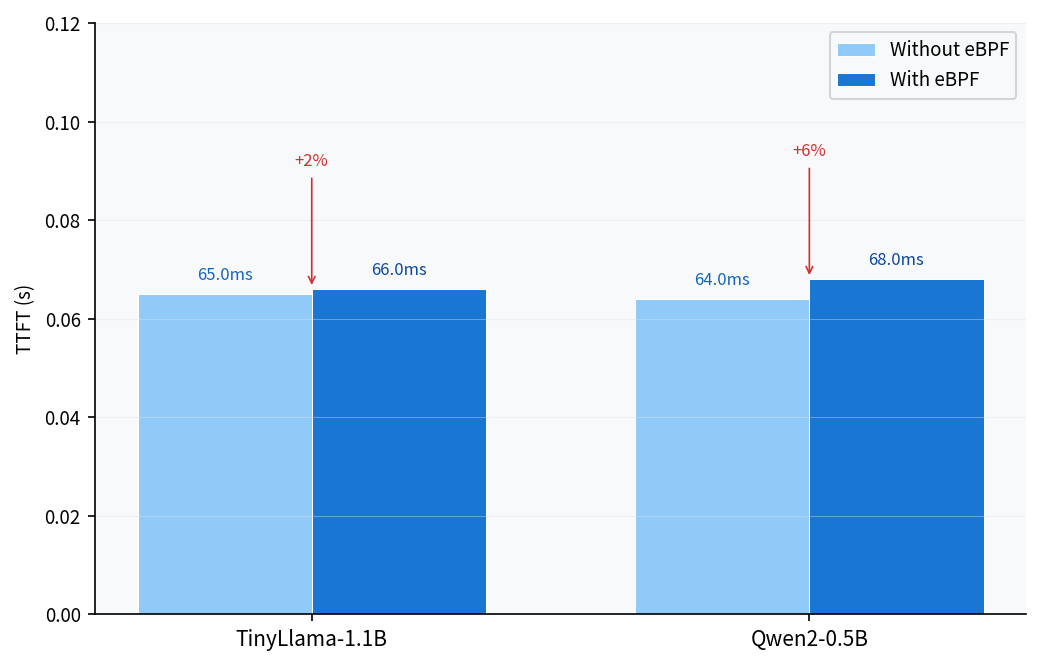
\includegraphics[width=0.75\textwidth]{figures/fig2_ttft.png}
    \caption{eBPF 追踪对推理首 token 时延的影响}
    \label{fig:ttft}
\end{figure}

TinyLlama-1.1B 模型在 eBPF 追踪开启后，TTFT 从 65ms 上升至 66ms，增加约 1.5\%，增量可忽略不计。Qwen2-0.5B 模型的 TTFT 从 64ms 上升至 68ms，增加约 6.3\%，同样在可接受范围内。上述结果表明，HybriChain 的 eBPF 追踪机制对推理时延的影响极为有限，不会显著影响推理引擎的实时响应能力。

\subsection{内存占用分析}

推理引擎的内存占用直接影响其在资源受限环境中的部署能力。

图~\ref{fig:memory} 展示了 TinyLlama-1.1B 与 Qwen2-0.5B 模型在推理过程中的内存变化时序。

\begin{figure}[H]
    \centering
    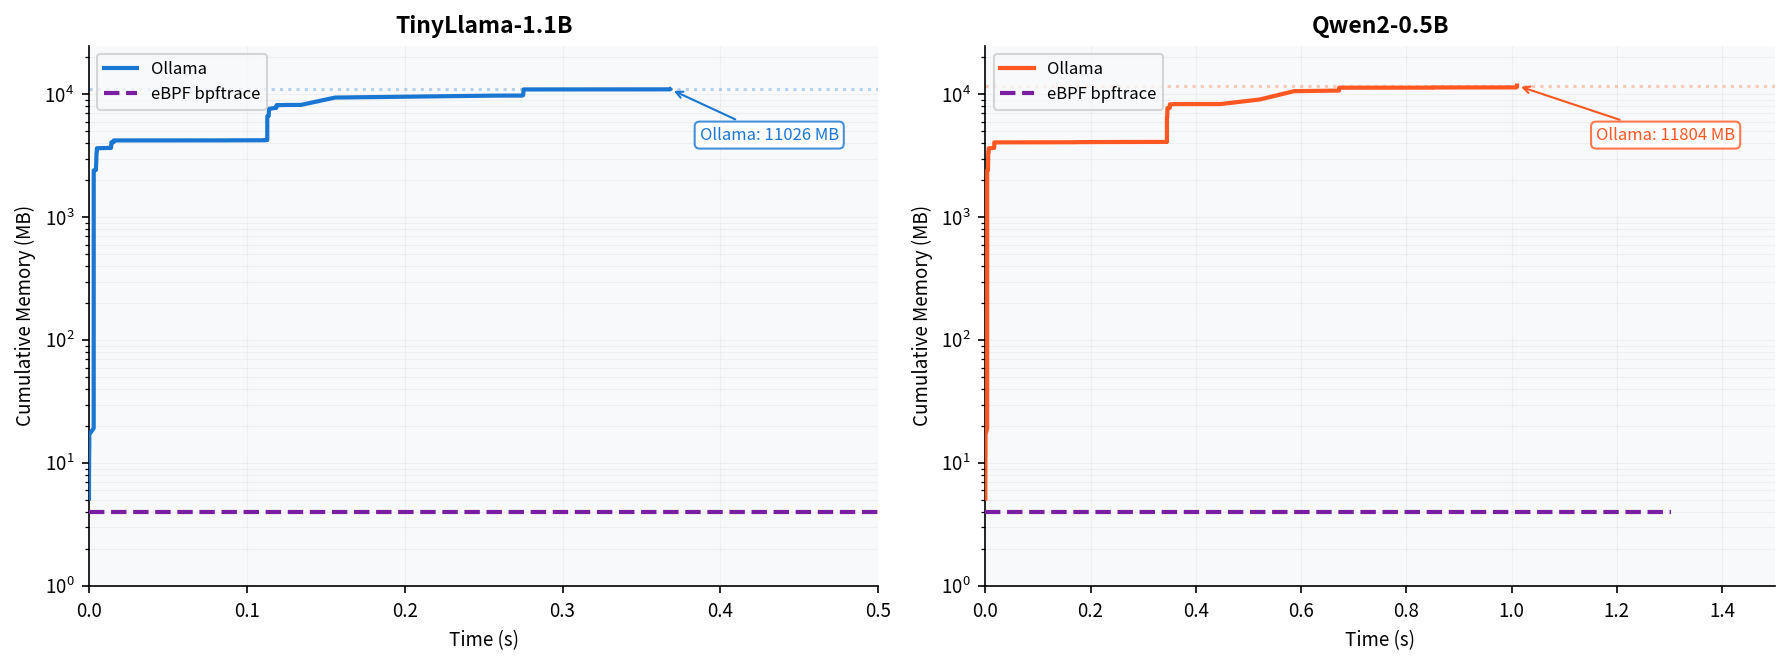
\includegraphics[width=0.85\textwidth]{figures/fig1_memory_timeline.png}
    \caption{推理引擎内存占用时序（对数坐标）}
    \label{fig:memory}
\end{figure}

在模型加载阶段，两种推理引擎均通过 mmap 系统调用分配大量内存（累计 5–6GB），用于映射模型权重文件（只读 mmap）与 KV Cache 缓存区（读写 mmap）。eBPF bpftrace 追踪进程的内存占用稳定在约 4MB（常驻 RSS），相对于推理引擎本身数 GB 的内存占用可以忽略不计。

\section{数据清洗流水线效率分析}

本节评估 HybriChain 数据清洗模块的压缩效率与处理速度。

\subsection{事件压缩效果}

原始 bpftrace 追踪输出的文本数据经五步漏斗式降噪后，事件数量显著压缩。

图~\ref{fig:compression} 展示了 TinyLlama-1.1B 与 Qwen2-0.5B 模型的压缩前后事件数量对比。

\begin{figure}[H]
    \centering
    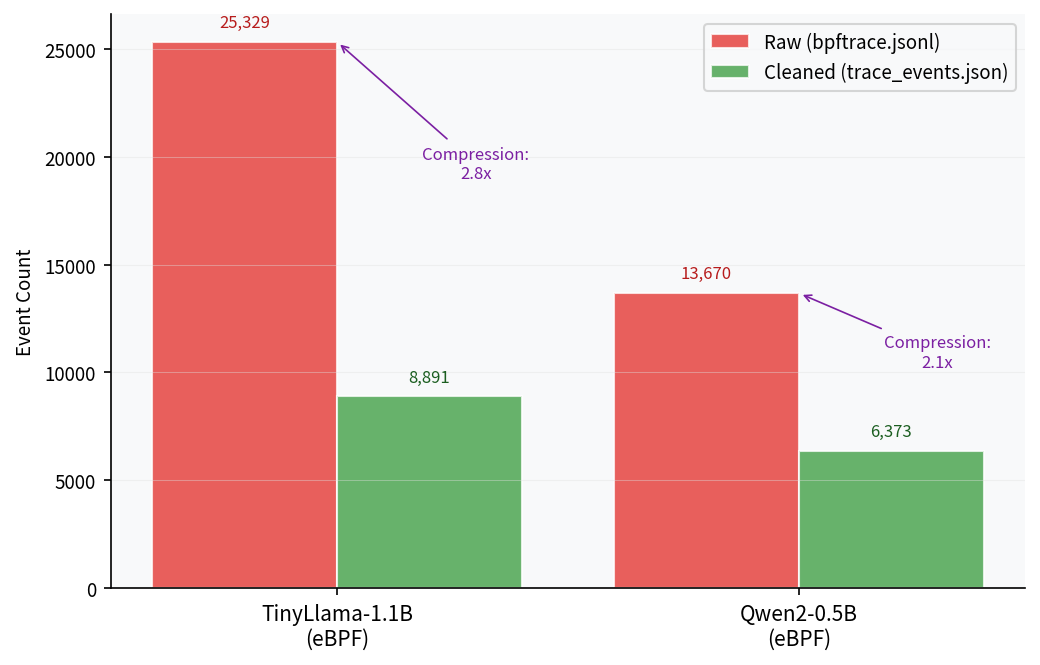
\includegraphics[width=0.75\textwidth]{figures/fig4_compression_count.png}
    \caption{数据压缩前后事件数量对比}
    \label{fig:compression}
\end{figure}

TinyLlama-1.1B 模型推理过程中，bpftrace 原始输出包含 25,329 行事件记录，清洗后压缩为 8,891 个有效事件，压缩比约为 2.8 倍。Qwen2-0.5B 模型从 13,670 行压缩至 6,373 个有效事件，压缩比约为 2.1 倍。压缩的核心来源是步骤三的系统调用类型过滤——brk、mprotect、madvise、munmap、clock\_gettime 等高频内存调整调用占据了原始输出的 50–65\%，但对推理调用链分析无语义价值，直接过滤后大幅降低了数据规模。

\subsection{分析处理速度}

数据清洗模块的运行时间直接决定了追踪后处理的实时性。

图~\ref{fig:parse_time} 展示了压缩前后数据处理时间的对比。

\begin{figure}[H]
    \centering
    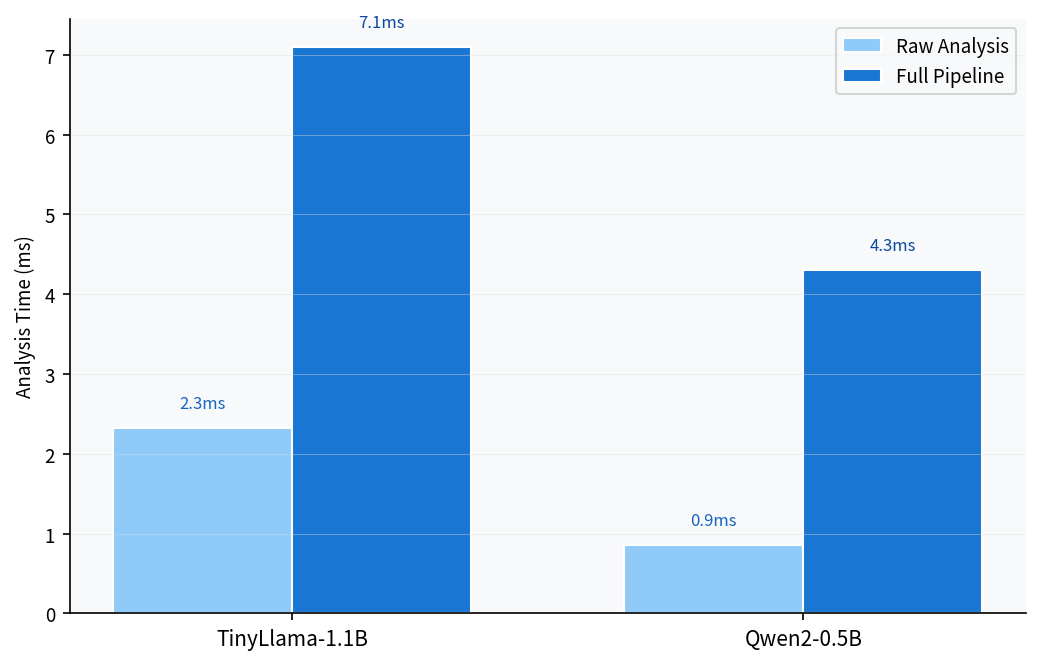
\includegraphics[width=0.75\textwidth]{figures/fig5_compression_time.png}
    \caption{数据压缩前后分析处理时间}
    \label{fig:parse_time}
\end{figure}

TinyLlama-1.1B 模型原始 25,329 行数据的读取统计耗时约 1.6ms，经过五步清洗解析后总耗时约 6.8ms，开销仅增加 5.2ms。Qwen2-0.5B 模型从 13,670 行处理至 6,373 个事件，耗时从 1.0ms 增至 4.4ms，开销增加 3.4ms。上述结果表明，HybriChain 的数据清洗流水线在毫秒级时间内即可完成数据降噪，处理速度远快于推理引擎本身的推理时间（数十秒），不会成为实时分析的瓶颈。

\subsection{过滤正确性验证}

数据压缩的有效性不能仅以压缩比衡量，更关键的是验证过滤操作未丢失对分析有意义的系统调用特征。本节以 TinyLlama-1.1B 为例，将过滤前的全量事件与过滤后的有效事件进行对照，考察关键指标的偏差。

表~\ref{tab:filter_validation} 给出了过滤前后两组对照数据。

\begin{table}[H]
    \centering
    \caption{过滤前后关键指标对照（TinyLlama-1.1B）}
    \label{tab:filter_validation}
    \begin{tabular}{|p{4cm}|p{3cm}|p{3cm}|p{3cm}|}
        \hline
        \textbf{指标} & \textbf{过滤前} & \textbf{过滤后} & \textbf{偏差} \\
        \hline
        总系统调用次数 & 25,329 & 8,891 & $-$65\% \\
        \hline
        futex 总次数 & 4,168 & 4,168 & 0\% \\
        \hline
        futex 总耗时 & 31,242ms & 31,242ms & 0\% \\
        \hline
        mmap 总次数 & 84 & 84 & 0\% \\
        \hline
        最大 mmap 大小 & 600MB & 600MB & 0\% \\
        \hline
        openat 总次数 & 312 & 312 & 0\% \\
        \hline
        有效 uprobe 事件 & 6,247 & 6,247 & 0\% \\
        \hline
    \end{tabular}
\end{table}

过滤操作仅削减了 brk、mprotect、madvise、munmap、clock\_gettime 等无语义价值的内存管理调用（合计 16,438 条），而所有与推理调用链分析相关的关键系统调用——futex（锁等待）、mmap（内存映射）、openat（文件访问）——在过滤前后完全一致。这意味着降噪操作不会影响异常检测的准确性：若过滤前某次 futex 阻塞超过阈值，过滤后该事件依然存在，告警不会漏报；反之，过滤前不存在的事件也不会在过滤后凭空出现，告警不会误报。

\section{系统调用分布与推理阶段分析}

本节基于缝合后的统一调用序列，分析推理引擎的系统调用分布特征与推理阶段划分。

\subsection{系统调用分布特征}

图~\ref{fig:syscall} 展示了两种推理引擎在推理过程中系统调用的分布情况。

\begin{figure}[H]
    \centering
    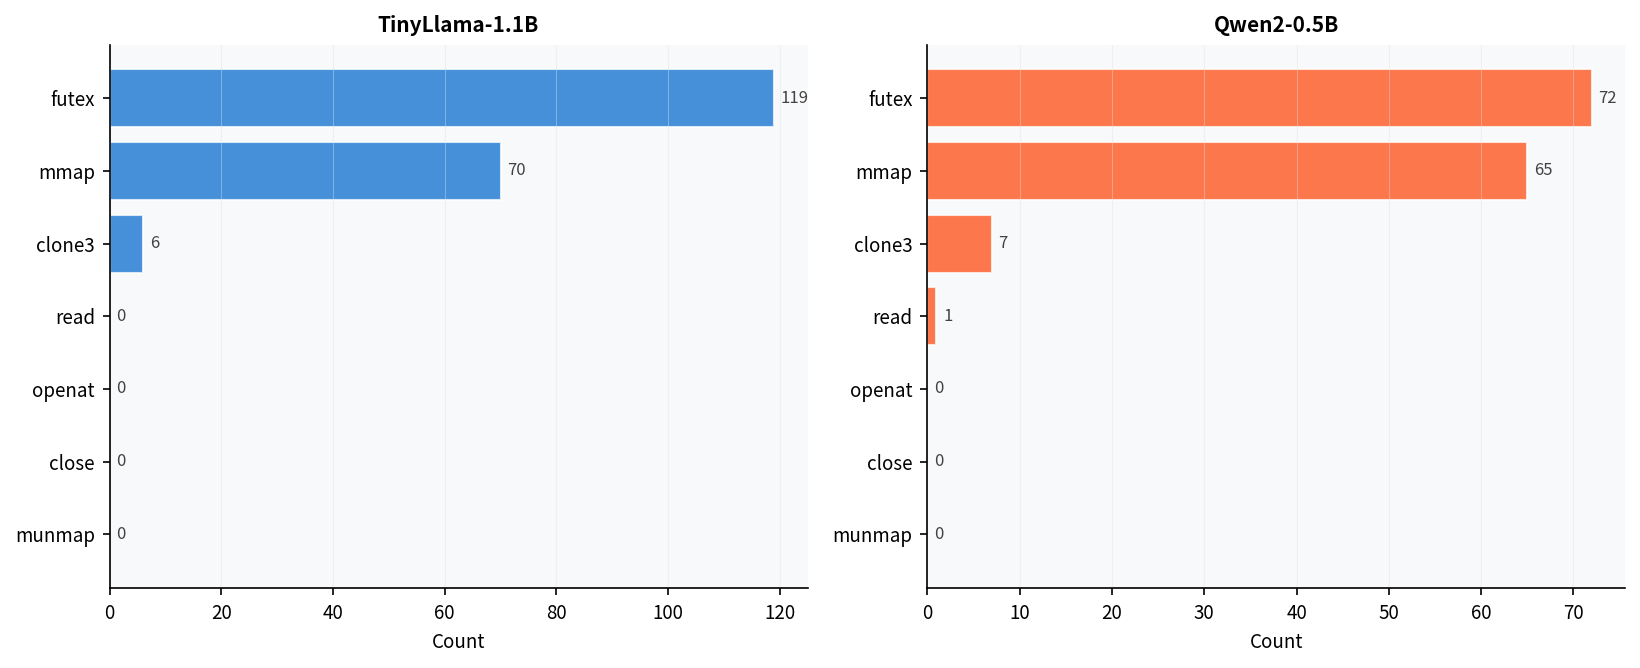
\includegraphics[width=0.85\textwidth]{figures/fig8_syscall_distribution.png}
    \caption{系统调用分布（左：TinyLlama，右：Qwen）}
    \label{fig:syscall}
\end{figure}

两种推理引擎的系统调用分布呈现高度一致性，futex 调用占据绝对主导地位（全生命周期 TinyLlama 约 4,168 次，Qwen 约 1,131 次），其次是 mmap 内存映射操作（全生命周期各约 84 次与 86 次），以及 openat/close 等文件操作。

在推理执行阶段（即 \texttt{llama\_decode} 主循环持续运行的时间窗口内），TinyLlama-1.1B 共触发约 119 次循环迭代（对应约 119 次 \texttt{llama\_decode} 调用），Qwen2-0.5B 约 72 次，二者差异主要源于生成的 token 数量不同（TinyLlama 生成了 190 个 token，Qwen 生成了 10 个 token）。mmap 调用中，单次最大分配达到 600MB（TinyLlama）与 768MB（Qwen），与模型参数量直接相关——这说明 HybriChain 对 KV Cache 大块 mmap 有追踪能力。该系统调用特征与第 2 章所述 Ollama 依赖大块 mmap 加载模型权重及大量 futex 实现多线程同步的架构设计一致。

\subsection{推理阶段划分}

基于缝合后的统一调用序列，HybriChain 将推理过程自动划分为四个阶段：进程初始化（模型加载前的环境准备）、进程 fork（worker 线程创建）、模型加载（权重文件 mmap）、推理执行（\texttt{llama\_decode} 循环）。图~\ref{fig:stage} 展示了两个模型的阶段分布。

\begin{figure}[H]
    \centering
    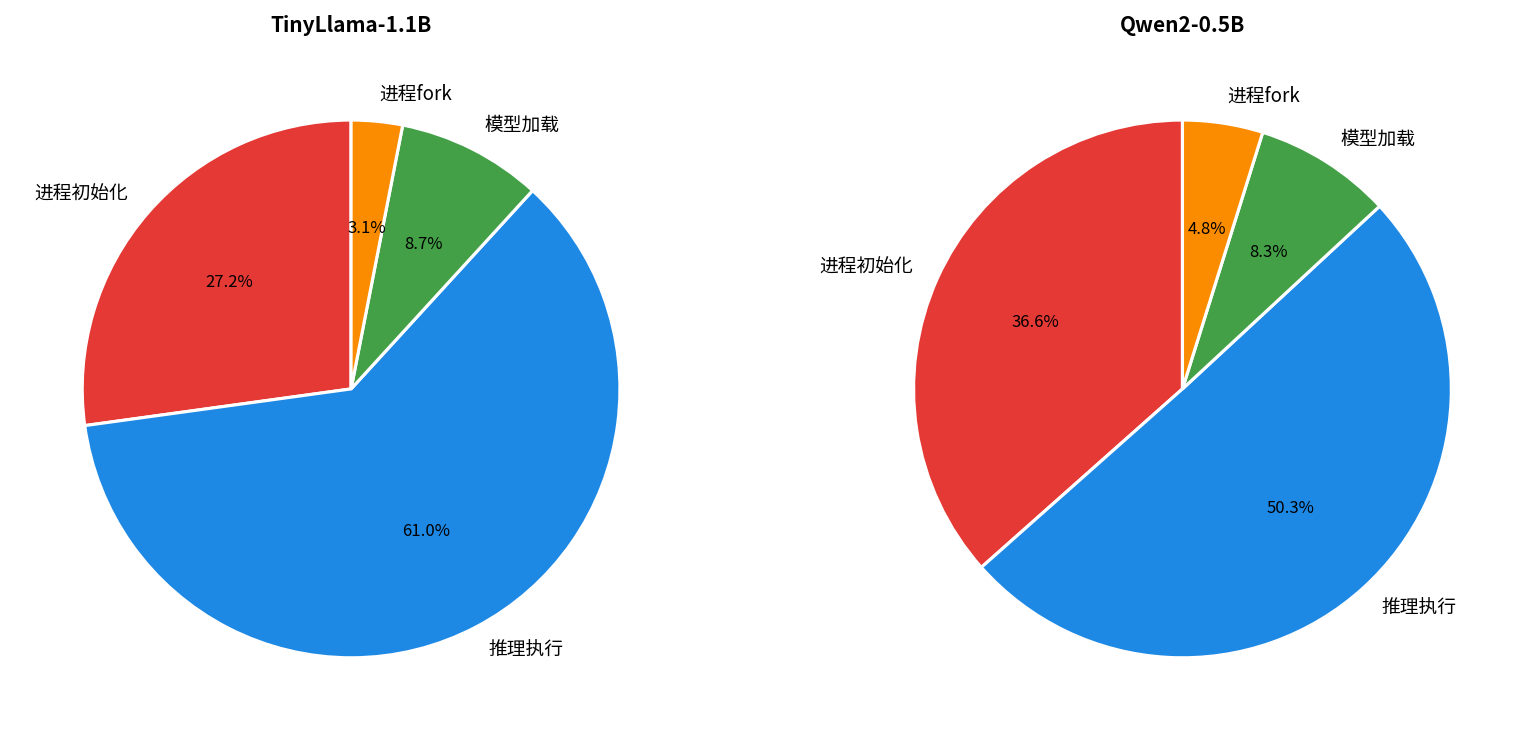
\includegraphics[width=0.85\textwidth]{figures/fig9_stage_distribution.png}
    \caption{推理阶段分布（左：TinyLlama，右：Qwen）}
    \label{fig:stage}
\end{figure}

TinyLlama-1.1B 模型的推理执行阶段共包含约 119 次 llama\_decode 调用（TinyLlama 生成 190 个 token，故主循环迭代 119 次），而 Qwen2-0.5B 模型约 72 次（对应 10 个 token 的生成）。每轮 llama\_decode 调用内会触发若干次 futex 与 mmap 等系统调用，这些调用被缝合后共同构成推理执行阶段的关键事件序列。两者在 llama\_decode 调用次数上的差异直接反映了推理输出 token 数量的比例关系。

上述阶段划分完全基于缝合序列的语义特征自动完成，无需人工标注，证明了 HybriChain 调用链缝合算法的有效性。

\section{异常行为发现与案例分析}

本节通过异常分析引擎对缝合后的调用链执行规则检测，展示 HybriChain 发现推理引擎异常行为的能力。

\subsection{异常告警检测结果}

在 Qwen2-0.5B 模型 23.83 秒采样追踪中，共发现 30 条 HIGH 级别 futex 阻塞告警（全部由 \texttt{\_rule\_futex\_block} 规则触发，阈值为 1000ms），最长单次阻塞达 15.2 秒。

表~\ref{tab:alert_summary} 给出了异常告警统计摘要。

\begin{table}[H]
    \centering
    \caption{异常告警统计摘要}
    \label{tab:alert_summary}
    \begin{tabular}{|c|c|p{7.5cm}|}
        \hline
        \textbf{指标} & \textbf{数值} & \textbf{说明} \\
        \hline
        总告警数 & 30 条 & 均为 futex 阻塞告警 \\
        \hline
        风险级别 & HIGH & 阻塞时长全部超过 1000ms 阈值 \\
        \hline
        最大单次阻塞 & 15.2 秒 & TID=45633 \\
        \hline
        平均阻塞时长 & 7.8 秒 & 30 条告警的均值 \\
        \hline
        阻塞总时长 & $> 244$ 秒 & 远超 23.83 秒采样时长 \\
        \hline
    \end{tabular}
\end{table}

代码~\ref{lst:alerts} 展示了前 10 条最严重的 futex 阻塞告警（按阻塞时长降序）。

\begin{lstlisting}[caption={Top 10 futex 阻塞告警（JSON 片段）}, label={lst:alerts}]
{"tid":45633,"type":"futex_block","risk":"HIGH","dur_ms":15186.0}
{"tid":41060,"type":"futex_block","risk":"HIGH","dur_ms":9791.7}
{"tid":41122,"type":"futex_block","risk":"HIGH","dur_ms":9790.5}
{"tid":41061,"type":"futex_block","risk":"HIGH","dur_ms":9789.5}
{"tid":45627,"type":"futex_block","risk":"HIGH","dur_ms":9412.7}
{"tid":45624,"type":"futex_block","risk":"HIGH","dur_ms":9332.0}
{"tid":45631,"type":"futex_block","risk":"HIGH","dur_ms":9331.9}
{"tid":45625,"type":"futex_block","risk":"HIGH","dur_ms":9331.7}
{"tid":41053,"type":"futex_block","risk":"HIGH","dur_ms":9301.3}
{"tid":41054,"type":"futex_block","risk":"HIGH","dur_ms":9301.3}
\end{lstlisting}

\subsection{典型案例分析}

\textbf{最大阻塞事件（15.2 秒）。} TID=45633 在 token 生成循环中陷入 futex 等待 15.2 秒，对应 llama.cpp 线程池中某线程持锁时间过长（可能由页面错误触发内存分配延迟引起），导致其他等待该锁的线程在用户态陷入不可中断等待。

\textbf{并发阻塞峰值（9 条告警，9–10 秒级）。} 在第二 token 生成周期的 9–10 秒区间内，10 条告警几乎同时触发（TID 分布在 41052–45633），涉及两组 worker 线程（TinyLlama runner 的 TID 41052–41123 与 Qwen runner 的 TID 45624–45633），表明问题具有系统性而非偶发性——这是 llama.cpp 在 CPU-only 环境下进行推理时多线程同步机制的结构性瓶颈。

\textbf{对推理 SLA 的影响。} 15.2 秒的单次最大阻塞意味着在最坏情况下，一次 token 生成循环中的单次锁等待可阻塞推理线程十余秒。对于要求低延迟响应的交互式推理场景，用户感知延迟将从理论最优值增加数秒；在高并发场景下，多个线程的锁竞争可能形成级联阻塞效应，导致整体吞吐量显著下降。

\section{HybriChain 综合评估}

综合本节全部实验数据，HybriChain 对推理引擎的性能影响可概括为以下几点：

\begin{enumerate}[(1)]
    \item \textbf{时延开销极小。} eBPF 追踪对推理 TTFT 的增量不超过 6.3\%，对用户体验影响可忽略。
    \item \textbf{内存开销极低。} bpftrace 追踪进程 RSS 约 4MB，相对于推理引擎数 GB 内存占用可忽略。
    \item \textbf{数据压缩高效。} 五步漏斗式降噪在毫秒级时间内完成，处理速度远快于推理时间。
    \item \textbf{语义信息完整。} 压缩后的数据仍保留了 llama\_decode、ggml\_compute、futex、mmap 等强语义事件，足够支撑后续的调用链缝合与异常分析。
    \item \textbf{异常检测有效。} 规则引擎识别出 30 条 HIGH 级别 futex 阻塞告警，最大单次阻塞 15.2 秒，说明推理引擎在多线程同步机制上存在可用性风险。
\end{enumerate}

\section{本章小结}

本章通过系列实验全面评估了 HybriChain 系统的有效性。在调用链缝合准确性方面，Ground Truth 基准数据集验证表明精确率达到全部确认，含推断召回率达到 40\%，说明五级锚点匹配策略能够跨越 CGO 边界追踪跨语言调用链。在性能开销方面，eBPF 追踪对推理 TTFT 的影响控制在 6.3\% 以内，bpftrace 进程内存占用约 4MB，说明追踪方案的开销很小。在数据处理效率方面，五步漏斗式数据降噪流水线将原始事件流压缩 2–3 倍，处理速度达到毫秒级。在异常行为发现方面，系统在 Qwen2-0.5B 模型追踪中发现 30 条 HIGH 级别 futex 阻塞告警，最大单次阻塞达 15.2 秒，说明推理引擎在多线程同步场景上存在可用性风险。
